\documentclass[10pt,letterpaper]{article}
\usepackage[utf8]{inputenc}
\usepackage[spanish,mexico]{babel}
\usepackage{amsmath}
\usepackage{amsfonts}
\usepackage{amssymb}
\usepackage{makeidx}
\usepackage{graphicx}
\usepackage{lmodern}
\usepackage{kpfonts}

\usepackage[left=2cm,right=2cm,top=2cm,bottom=2cm]{geometry}
% Entre signos de porciento se escriben un comentario%
% datos del autor y del reporte %
\author{Aldo Josué Huerta-Verde}
\title{Práctica 1, Título de la Práctica }
\begin{document}
\maketitle

\begin{abstract}
Descripción del trabajo realizado, resumido entre cincuenta y cien palabras.
\end{abstract}

\section{Introducción}
Aquí va la información relevante que ayudará al lector a entender el qué se hace y los métodos utilizados para el desarrollo del experimento. No debería ser más de una cuartilla de texto. \cite{intro_datos}% Esta es una cita de la bibliografía solo a modo de ejemplo, no tiene ninguna relación aquí.

\section{Objetivo}
¿Cuál es el objetivo u objetivos del experimento?
Por ejemplo.
Determinar experimentalmente el valor de la aceleración de la gravedad en la Ciudad de México.

\section{Hipótesis}
¿Qué esperaban obtener antes de iniciar el experimento?
El Valor de la aceleración de la gravedad en México es $9.779026\frac{m}{s^2}$ reportado en \cite{cenam_gravedad}.

\section{Material}
Lista de materiales usados, indicando Modelo y Marca de cada uno (Para efectos de reproducibilidad). \\
Una figura del montaje experimental también ayuda a entender lo que se hace.

\section{Método experimental}
Básicamente aquí describen los pasos que siguieron para la realización del experimento.

\section{Observaciones}
En ésta seccion describen los problemas que tuvieron, las condiciones en las que trabajaron, es decir, si realizaron en varios días sus muestreo, si usaron diferentes materiales cada vez, si tomaron los datos personas distintas cada vez etc.

\section{Análisis de datos}
Aquí colocan los datos que se obtuvieron, una tabla es la mejor forma de presentar datos. Describan que es cada tabla con Pies de tabla.
\begin{table}[ht!]
  \centering
  \begin{tabular}{|c|c|}
  \hline %pinta una línea horizontal en la tabla
  Tiempo (s) & Posición (m) \\
     \hline
     0.0&-0.040860998212862876 \\
0.033333333333333375&-0.03980424825908195\\
0.06666666666666668&-0.03769074835152007\\
0.1&-0.03416824850558363\\
0.13333333333333336&-0.028532248752085307\\
0.16666666666666663&-0.022543999013993316\\
0.20000000000000012&-0.016555749275901352\\
0.23333333333333336&-0.009158499599434794\\
0.2666666666666667&-0.0014089999383745944\\
0.3000000000000001&0.00598824973809195\\
\hline
  \end{tabular}
  \caption{Descripción de los datos de la tabla, por ejemplo, Datos de posición contra tiempo en la corrida 1 del resorte con masa $m$}
  \label{resortito} % esta es una etiqueta con la que pueden hacer referencia en cualquier parte del texto. 
\end{table}
\\
Si van a hacer alguna gráfica aquí iría también.
\\
\begin{figure}[ht!]
    \centering
    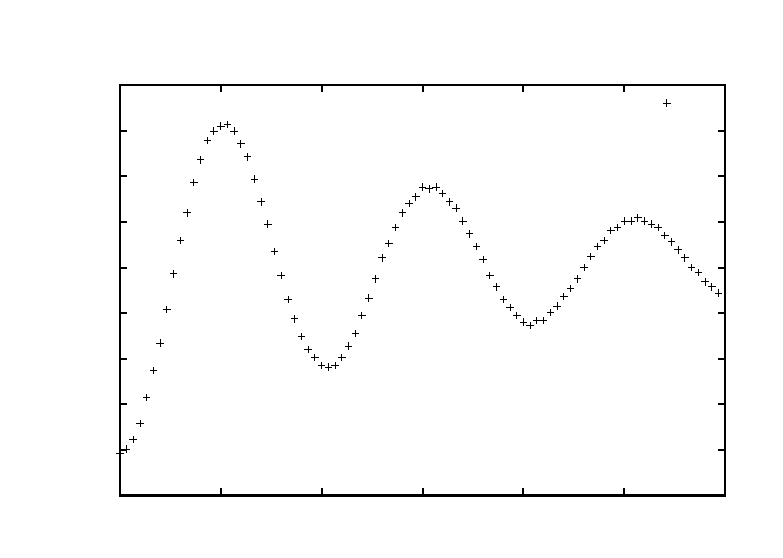
\includegraphics[scale=1]{resorte.eps} 
    \caption{Posición contra tiempo del resorte Datos de la Tabla \ref{resortito}} %aquí hacemos mención de la tabla que agregamos previamente 
    \label{fig:awesome_image}
\end{figure}



\section{Resultados}
Aquí reportan los datos que obtuvieron del análisis previo, pueden agregar gráficas de sus datos con los ajustes que relizaron.

\section{Conclusiones}
Aquí discutirán los resultados que obtuvieron, si pudieron validar la o las hipótesis que plantearon y porqué son válidos los mismos.
Recuerden que vamos a reportar valores conocidos, estremos validando durante éste curso, mediante experimentos, diversas constantes físicas; por lo tanto, presentar el resultado como un porcentaje entre el valor conocido y el que obtuvieron durante con el experimento. 


\begin{thebibliography}{9}

\bibitem{intro_datos}
  Oda Noda, Bertha,
  \emph{Introduccion al análisis gráfico de datos experimentales}.
  Universidad Nacional Autónoma de México. Facultad de Ciencias,
  3ra edición,
  2005.
\bibitem {cenam_gravedad}
  Centro Nacional de Metrología, 
  \emph{Cálculo de la Aceleración Local de la Gravedad}. 
  http://www.cenam.mx/fyp/aceleracion.html
\end{thebibliography}

\end{document}